\chapter{Completed Work}


This work was published at Physical Review E \cite{de_leeuw_diffusion_2012},
and reprinted here in \autoref{sec:papers}. In the
following sections we will provide an overview
of the main results.


%%%%%%%%%%%%%%   Overview over article should not include too much equations
%%  bottom line - take home message - the derivations should ref the article

%%  
%%  remove the techinalities - 
%%     using the procedure we have calculated for.. blah blah
%%       see figure. (leave plots only if neccessary to buttom line).
%%
%%  geometry plots - maybe try with normal scale.
%%                   if that doesn't work, leave the figure out.



%%%%%%%%%%%%%%%%%%%%%%%%%

%%%%%%%%%%%%%
%\section{Article abstract}
%\rmrk{This is the article abstract..}


We have studied random networks whose dynamics are
described by a rate equation, with transition rates $w_{nm}$
that form a symmetric matrix (\autoref{sec:matrix_categories}),
with a diagonal conforming to \autoref{eq:zero_sum}. 
%
The long time evolution
of the system is characterized by a diffusion coefficient~$D$.
In one dimension it is well known that $D$ can display an abrupt
percolation-like transition from diffusion (${D>0}$)
to sub-diffusion (${D=0}$). 
%
A question arises whether
such a transition happens in higher dimensions.
Numerically $D$ can be evaluated using a resistor network
calculation, or optionally it can be deduced from 
the spectral properties of the system. Contrary to a recent 
expectation that is based on a renormalization-group analysis, 
we deduce that $D$ is finite.
%
We suggest an ``effective-range-hopping" procedure to evaluate $D$,
and contrast the results with the linear estimate.
The same approach is useful for the analysis of 
networks that are described by quasi-one-dimensional  
sparse banded matrices. 


%%%%%%%%%%%%%%%%%%%%%%%%%
\section{The effective range hopping procedure}


The basic idea behind \emph{ERH} (effective range hopping) is that in the linear
expression, nearby sites 
with $r\ll 1$ (and therefore $w \gg 1$ ) are over represented in
the diffusion coefficient calculation. While the transition to
these sites is indeed high, the distance covered is not enough
to form a percolating cluster. Therefore, we use a threshold based
on percolation theory and flat-down the rates higher then this threshold.
This produces a smooth crossover between the linear
estimate and the \emph{VRH} estimate.


Using the \emph{ERH} procedure we have calculated the diffusion for several models.


For the degenerate hopping model we obtained:

\begin{align}
D_{\tbox{ERH}} &=  \mathrm{EXP}_{d{+}2}\left(\frac{1}{s_c}\right)  \  \eexp{-1/s_c}  \ D_{\tbox{linear}}
\end{align}
%
For infinite dimensions ($d\rightarrow\infty$),  we have $\mathrm{EXP}_{d{+}2}\  \eexp{-1/s_c} = 1$. 
This means that the ERH expression converges with the linear expression.
For low dimensionality, the exponent dominant.


For the Mott Hopping model,
%
\begin{align}
D_{\tbox{ERH}} &=\mathrm{EXP}_{d{+}3}\left(\epsilon_c\right)  \  \eexp{-\epsilon_c}  \ D_{\tbox{linear}}
\end{align}
%


For the flat-profile banded $1d$ model,
\begin{align}
D_{\text{ERH}} \ \ &= \ \ 
\ \frac{1}{\sigma}\left[ 
\left(1+\frac{n_c}{2b}\sigma\right)\eexp{-\frac{n_c}{2b}\sigma} - \eexp{-2\sigma}
\right] \ \tilde{b} w_0 \\ &=\ \ 
\ \frac{\left(1+\frac{n_c}{2b}\sigma\right)\eexp{-\frac{n_c}{2b}\sigma} - \eexp{-2\sigma}}
       {1 - \eexp{-2\sigma}}
   \ D_{\tbox{linear}}
\end{align}



%%%%%%%%%%%%%%%%%%%%%%%%%%%%%%%%%%%%%%%%%%%%%%%%%%%%
%%%%%%%%%%%%%%%%%%%%%%%%%%%%%%%%%%%%%%%%%%%%%%%%%%%%
\chapter{Preliminary analysis}




%%%%%%%%   I need to add dts.tex here.
%%%%%%%%   I could also add D(g_s) and say that it failed

%%%%%%%%%%%%%%%%%%%%%%%%%%%%%%%%%%%%%%%%%%%%%%%%%%%
\section{A banded classical Hamiltonian}%PTA


We have analyzed a model of springs and masses described in \autoref{eq:app_heat}.
The Hamiltonian is quadratic in the $K$ matrix as defined in \autoref{eq:K_matrix},
which means that the eigenvalues $\lambda$ of $K$ determine the frequencies $\omega^2 = \lambda$.
The eigenvectors are of course the same.

In recent studies \cite{bodyfelt_unpub} an interesting structure of
PN (participation number) was observed in this model. 

As can be seen
in \autoref{fig:PN_kottos}, for the low eigenvalues, instead of the 
expected large PN, we have some decrease. After that, follows a period
of large PN, followed by another segment with somewhat smaller PN.
Another quantity we calculated is the Thouless conductance (see \autoref{sec:anderson}), 
which we expect to correlate with $PN$. Disregarding major numerical issues,
the correlation seems to hold, see \autoref{fig:PN_g_scatter}.

\notbool{showfigure}{\begin{comment}}{}

\begin{figure}[H]
  %\subfloat[Low sparsity]{
  \begin{subfigure}{.45\linewidth}\centering
    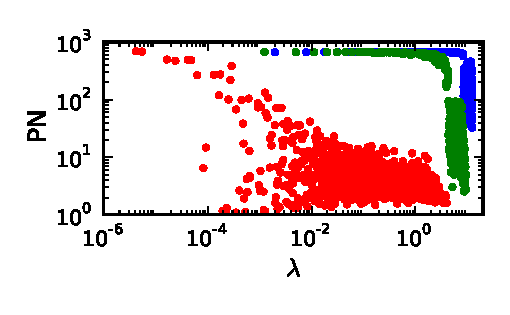
\includegraphics[width=0.99\linewidth]{pta_nopin}
    \caption{PN vs $\lambda$}\label{fig:PN_kottos_nopin}
  \end{subfigure}
  %
  \begin{subfigure}{.45\linewidth}\centering
     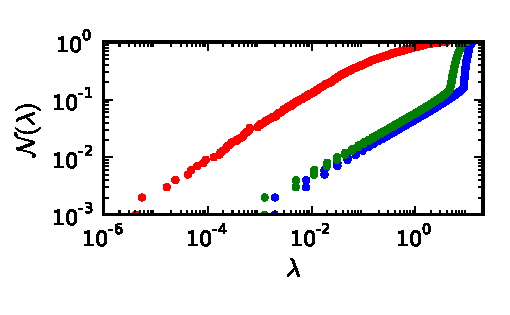
\includegraphics[width=0.99\linewidth]{pta_ev_nopin}
  \caption{Counting function (CDF) $\mathcal{N}(\lambda)$}\label{fig:ev_dist}
  \end{subfigure}\\ % end of row
  %
 % \caption{}
 % \end{figure}
 % \begin{figure}[H]
  %
    \begin{subfigure}{.45\linewidth}\centering
    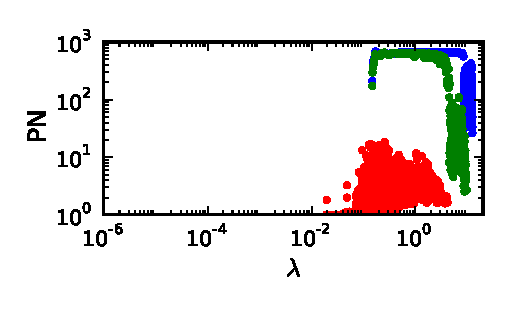
\includegraphics[width=0.99\linewidth]{pta_pin}
    \caption{PN vs $\lambda$, with diagonal disorder}\label{fig:PN_kottos_pinning}
  \end{subfigure}     
  %
  \begin{subfigure}{.45\linewidth}\centering
     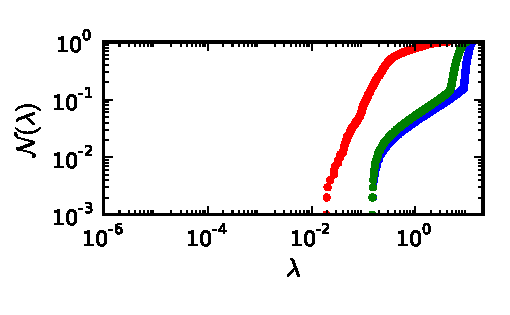
\includegraphics[width=0.99\linewidth]{pta_ev_pin}
  \caption{Counting function (CDF) $\mathcal{N}(\lambda)$ with diagonal disorder}\label{fig:ev_dist_pin}
  \end{subfigure}
    \begin{subfigure}{.45\linewidth}\centering
    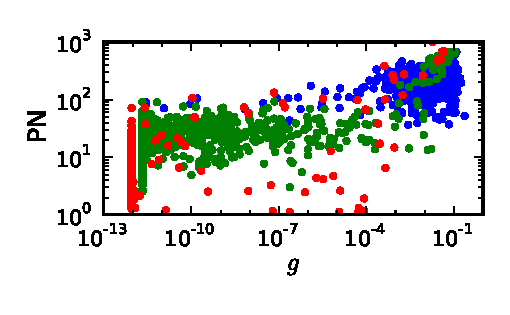
\includegraphics{pta_scatter_g}
  \caption{PN vs $g$}\label{fig:PN_g_scatter}
  \end{subfigure}
  \caption{For all the plots $N=1000$ and $b=5$. 
           In blue $\sigma=0.1$, green $\sigma=0.6$ and red $\sigma=10$, where higher
           $\sigma$ means more sparsity.
           %%%%
           In (\subref{fig:PN_kottos_nopin}) with low $\sigma$ (blue) we see two groups of PN values.
           This distinction is lost for higher $\sigma$ (red).
           %%
           In (\subref{fig:ev_dist}) we plot the cumulative distribution of
           the eigenvalues, presenting clear diffusive behavior, for any $\sigma$.
           %%%%%% pinning
           In (\subref{fig:PN_kottos_pinning}) and (\subref{fig:ev_dist})
           we see the effects of diagonal disorder (pinning)
           on the spectrum. We see clearly that the lowest eigenvalues 
           are affected, and their corresponding PN is much lower.
           %%%g 
           In (\subref{fig:PN_g_scatter}) we compare the Thouless conductance
           $g$ with the participation number. 
           The presented points do seem to be correlated, but due to numerical issues,
           many values of $g$ are below the precision limit (seen as a vertical line in the plot), 
           up to $936$ from $1000$ for $\sigma=10$. 
  }
\end{figure}

\notbool{showfigure}{\end{comment}}{}






%%%%%%%%%%%%%%%%%%%%%%%%%%%%%
\section{Quantum spreading in the quasi one dimensional Hamiltonian}

In this section the numerical work was done by our collaborators,
Eli Halperin and Tsampikos Kottos of Wesleyan university.

In this model , described in \autoref{sec:quasi_bg}, initial analysis of
the numerical results reveals that the sparsity affects the diffusion coefficient.
We see that as the system becomes more sparse, the diffusion coefficient is suppressed. 
As might be expected, the lower bandwidth ensembles are more
susceptible, as the system is more vulnerable to disconnections.


\begin{figure}
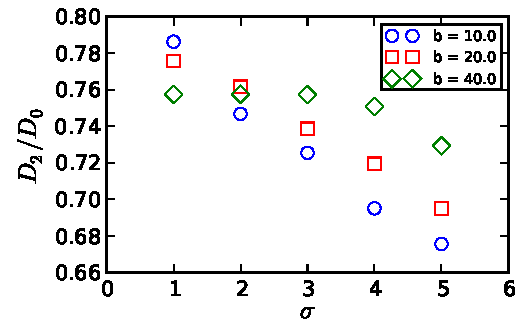
\includegraphics{dts_D2}
\caption{The transient diffusion coefficient for quantum spreading in
a banded sparse network. The ratio $D/D_0$ between the numerical diffusion 
coefficient and the expected value decreases as $\sigma$ increases. The effect
is stronger for low bandwidth.}
\end{figure}


Our first question was whether our rate equation analysis might
hold also for the quantum case, because in first order perturbation theory,
the transition probability $p_{nm}$ is proportional to $\left|\bra n|\mathcal{H} | m \ket\right|^2$.
Naively using our previously obtained suppression factor $g_s = \frac{D_{ERH}}{D_{\textrm{linear}}}$,
did not prove to be sufficient, as can be seen in \autoref{fig:d_vs_g}.

\begin{figure}
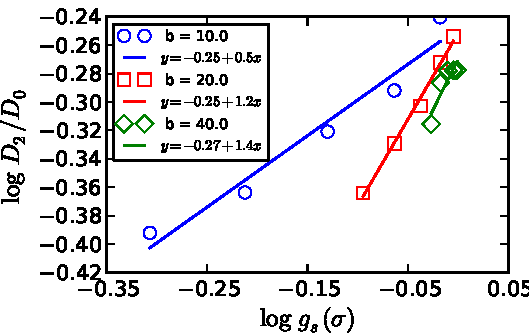
\includegraphics{dts_D2_vs_gs_loglog}
\caption{Scaled $D$ vs $g_s$. }\label{fig:d_vs_g}
\end{figure}
